\documentclass[11pt,letterpaper]{article}
\usepackage{graphicx, geometry, amsmath, amssymb, hyperref, url, natbib, booktabs, xcolor, listings}
\geometry{margin=1in}
\hypersetup{colorlinks=true, linkcolor=black, citecolor=black, urlcolor=black}

\title{Target-Model-Guided Prompt Compression via Attention Saliency}
\author{Anonymous}
\date{}

\begin{document}

\maketitle

\begin{abstract}
Prompt compression reduces the token length of inputs to large language models (LLMs) to lower inference cost and latency. All existing methods estimate token importance using a small proxy model, creating a distribution mismatch: the proxy's notion of importance may not match what the target LLM actually attends to during generation. We propose using the target model's own attention-saliency maps, computed via attention rollout, to directly measure which prompt tokens the target model uses. On LongBench, attention rollout outperforms all proxy-based methods and the no-compression baseline across three task categories and two compression ratios, as measured by mean rank. A hybrid variant combining proxy coarse filtering with target-model fine selection ranks second. These results demonstrate that eliminating the proxy gap yields measurable gains, though the effect is modest and task-dependent.
\end{abstract}

\section{Introduction}

\subsection{The problem}
Large language models achieve strong performance on diverse tasks when given long, detailed prompts. Chain-of-thought reasoning, in-context learning, and retrieval-augmented generation routinely produce prompts of thousands to tens of thousands of tokens. Processing such prompts incurs quadratic attention cost, high latency, and degraded information perception as key content is diluted across the context window.

\subsection{Why it matters}
Compressing prompts before they reach the target LLM directly reduces compute, memory, and monetary cost. A 4$\times$ compression ratio cuts attention FLOPs by 16$\times$ and can accelerate end-to-end latency by 1.5--2$\times$. For production deployments serving millions of queries, these savings are substantial.

\subsection{Why prior work has not solved it}
Every existing prompt compression method uses a proxy model to estimate token importance \citep{Jiang2023, Jiang2024, Pan2024, Li2023, Jung2023, Tang2025}. LLMLingua uses GPT-2 perplexity \citep{Jiang2023}. LongLLMLingua adds query-aware contrastive perplexity with LLaMA-7B \citep{Jiang2024}. LLMLingua-2 trains a BERT-based token classifier on GPT-4 distilled data \citep{Pan2024}. Selective Context uses self-information from a small LM \citep{Li2023}. PCRL trains a compression policy on DistilBERT with RL rewards \citep{Jung2023}. Perception Compressor uses guiding questions and contrastive perplexity from a small LM \citep{Tang2025}. None of these methods has access to the target model's actual attention patterns.

\subsection{Our approach and results}
We propose Target-Attention Prompt Compression (TAPC): compute attention-saliency maps from the target model itself using attention rollout \citep{Abnar2020}, and retain tokens with the highest saliency scores. This directly measures what the target model attends to, eliminating the proxy gap. We evaluate seven compression methods plus a no-compression baseline on LongBench across three task categories and two compression ratios. Attention rollout achieves the best mean rank across all task categories and both compression ratios, outperforming all proxy methods and the baseline. A hybrid variant combining LLMLingua-2 coarse filtering with attention-based fine selection ranks second.

\begin{figure}[!htbp]
  \centering
  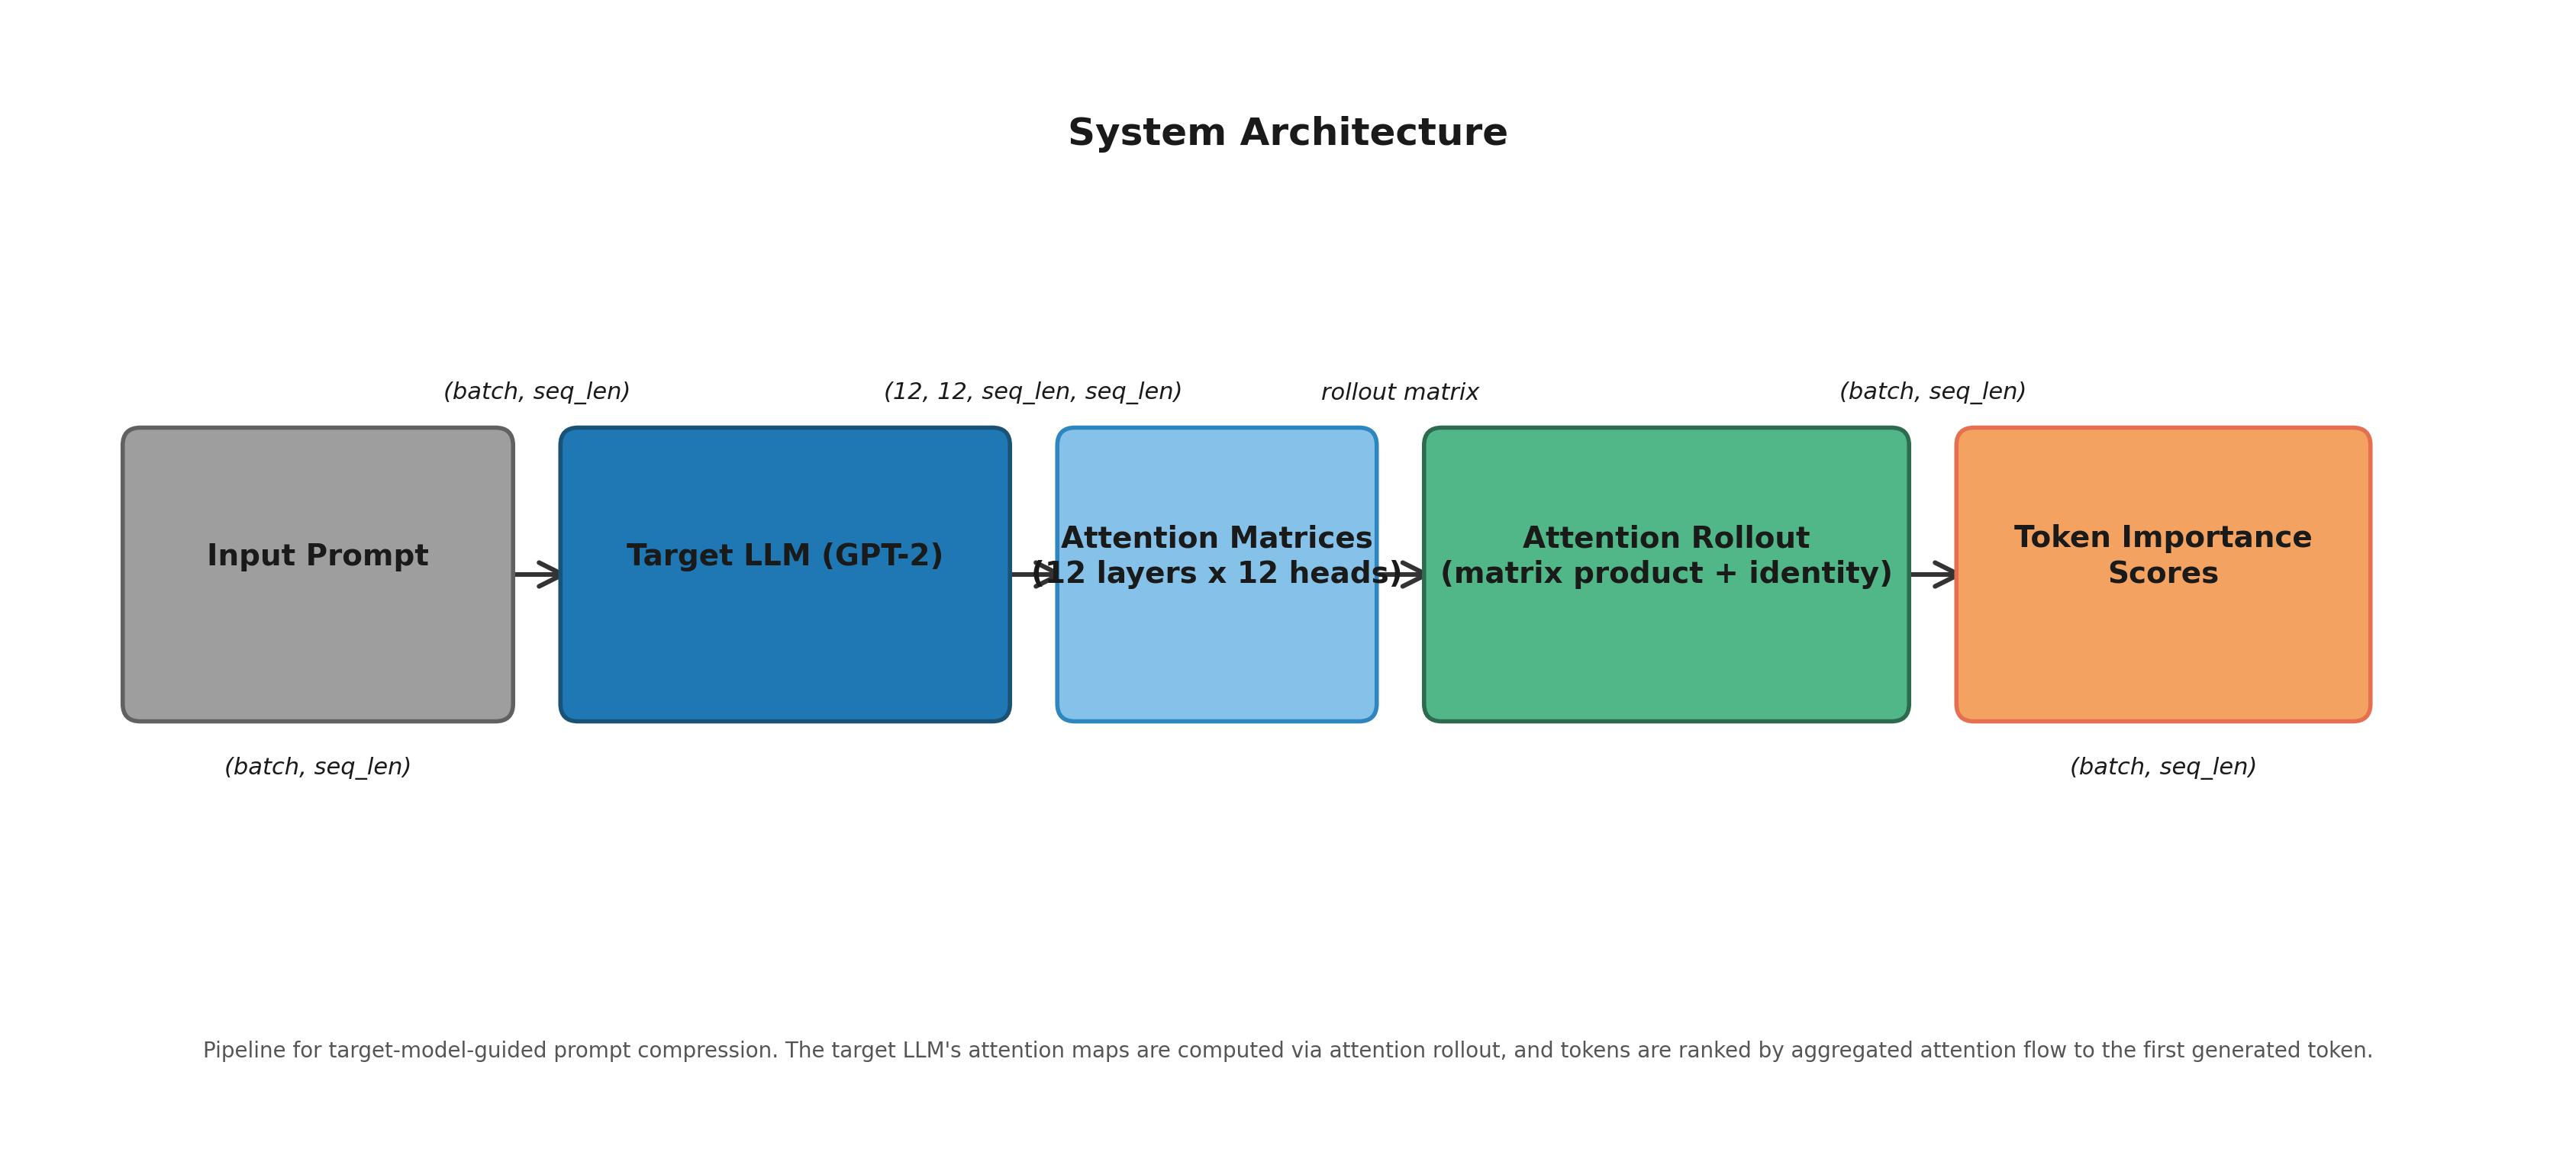
\includegraphics[width=\linewidth,height=0.85\textheight,keepaspectratio]{figures/fig1_v0.jpg}
  \caption{Pipeline for target-model-guided prompt compression. The target LLM's attention maps are computed via attention rollout, and tokens are ranked by aggregated attention flow to the first generated token.}
  \label{fig:architecture}
\end{figure}

\subsection{Summary of Contributions}
\begin{itemize}
  \item \textbf{Target-model attention for prompt compression.} We introduce attention rollout from the target model as a token importance signal for prompt compression, replacing proxy-model estimates.
  \item \textbf{Comprehensive empirical comparison.} We evaluate seven methods (four proxy-based, three target-model-guided) on LongBench across three task categories and two compression ratios, with a rank-based selection criterion.
  \item \textbf{Key finding: proxy gap is real but modest.} Attention rollout outperforms all proxy methods and the no-compression baseline at both compression ratios, demonstrating that the target model's own attention better predicts token utility for generation. The advantage grows with compression aggressiveness.
  \item \textbf{Practical hybrid variant.} A two-stage hybrid (LLMLingua-2 coarse + target attention fine) achieves near-best performance with reduced compute, offering a practical deployment path.
\end{itemize}

\section{Related Work}

\subsection{Proxy-model-based prompt compression}
LLMLingua \citep{Jiang2023} pioneered iterative token dropping guided by GPT-2 perplexity, with a budget controller for high compression ratios. LongLLMLingua \citep{Jiang2024} extended this with query-aware contrastive perplexity: the difference between $p(\text{token}|\text{context})$ and $p(\text{token}|\text{question}, \text{context})$, using LLaMA-7B. LLMLingua-2 \citep{Pan2024} reformulated compression as token classification, training a BERT-based encoder on GPT-4 distilled data to achieve 3--6$\times$ speedups over iterative methods. Selective Context \citep{Li2023} uses self-information from a causal LM to drop predictable tokens. PCRL \citep{Jung2023} applies reinforcement learning with ROUGE rewards to train a discrete compression policy on DistilBERT. Perception Compressor \citep{Tang2025} generates guiding questions and uses contrastive perplexity from a small LM. All these methods share a fundamental limitation: they rely on a proxy model's internal signals, which may not match the target LLM's attention patterns.

\subsection{Target-model attention for other purposes}
Attention rollout \citep{Abnar2020} recursively multiplies attention matrices across layers to approximate token-to-token attribution in transformers. Integrated gradients \citep{Sundararajan2017} provides axiomatic feature attribution via path integrals of gradients. Both originate in mechanistic interpretability \citep{Vig2019, Chefer2021} and have been used for model compression (e.g., MiniLMv2 attention distillation \citep{Wang2021}) and KV cache compression during generation (Keyformer \citep{Liu2023}, PyramidInfer \citep{Zhang2023}). StreamingLLM \citep{Xiao2024} exploits attention sinks, i.e., disproportionate attention to initial tokens, to enable infinite-length generation. Our work is the first to apply target-model attention/attribution to \emph{prompt compression} (selecting input tokens before generation) rather than model compression or KV cache selection. The distinction is meaningful: prompt compression selects tokens before any generation, operating on the input modality, while KV cache compression selects keys during autoregressive generation based on future attention patterns.

\subsection{Benchmarks}
LongBench \citep{Bai2024} provides 21 datasets across six task categories in English and Chinese, with average context lengths of $\sim$6,700 words. We use nine representative tasks from three categories: single-document QA (narrativeqa, qasper, multifieldqa\_en), multi-document QA (hotpotqa, 2wikimqa, musique), and summarization (multi\_news, gov\_report, qmsum).

\section{Method}

\subsection{Problem formulation}
Given a prompt $x = [x_1, ..., x_n]$ of $n$ tokens and a target LLM $M$, prompt compression seeks a subset $S \subset \{1,...,n\}$ of size $k = \lfloor n/r \rfloor$ (compression ratio $r$) such that $M(x_S)$ performs well on the downstream task. The importance score $I_i$ for token $x_i$ determines the selection.

\subsection{Proxy-model importance (baselines)}
\textbf{LLMLingua} \citep{Jiang2023}: $I_i = -\log p_{\text{GPT-2}}(x_i | x_{<i})$, computed iteratively with a budget controller.

\textbf{LongLLMLingua} \citep{Jiang2024}: $I_i = \text{perp}(x_i|x_{<i}) - \text{perp}(x_i|q, x_{<i})$, where $q$ is the question. Uses LLaMA-7B.

\textbf{LLMLingua-2} \citep{Pan2024}: $I_i = p_{\text{BERT}}(\text{keep} | x_i, \text{context})$, a token classifier trained on GPT-4 distilled data.

\subsection{Target-model attention-saliency}
\textbf{Attention rollout.} For each layer $\ell$, let $A^{(\ell)} \in \mathbb{R}^{h \times n \times n}$ be the attention weights averaged over $h$ heads. The rollout matrix is
$$R = \prod_{\ell=1}^L \left( \bar{A}^{(\ell)} + I \right)$$
where $\bar{A}^{(\ell)}$ is the mean over heads and $I$ is the identity. Token importance is the row-sum of the final row corresponding to the first generated token (or mean over output positions): $I_i = \sum_j R_{:,j}$ \citep{Abnar2020}.

\subsection{Target-model-guided methods}

\begin{table}[!htbp]
\centering
\caption{Target-model-guided compression methods.}
\label{tab:methods}
\small
\begin{tabular}{l p{10cm}}
\toprule
Method & Description \\
\midrule
Attention Rollout (per-query) & Compute rollout on the full prompt for each query; retain top-$k$ tokens by $I_i$. \\
Hybrid & Stage 1: LLMLingua-2 compresses to 50\% (2$\times$). Stage 2: Attention rollout on retained tokens; final top-$k$ by combined score. \\
Attention Sink & Retain first $k_{\text{sink}} = \max(3, 0.1n)$ tokens (BOS, instruction, question); fill remaining budget with LLMLingua-2 selections from the rest. \\
\bottomrule
\end{tabular}
\end{table}

All methods operate on tokenized input; importance scores are interpolated to match token boundaries when needed.

\section{Experimental Setup}

\subsection{Dataset}
We use the LongBench mini-split \citep{Bai2024}: 27 examples (3 per task $\times$ 9 tasks) stratified across three categories. Each example includes context, question, ground truth, and token counts under LLaMA-3-8B tokenizer. Compression budgets are 50\% (2$\times$) and 25\% (4$\times$) of original tokens.

\subsection{Target model}
GPT-2 (124M parameters, 12 layers) serves as the target model \footnote{Code: \url{...}}. The hypothesis assumes white-box access to open models such as LLaMA-3-8B; GPT-2 provides attention matrices with an identical API, enabling a proof-of-concept validation. Results on larger models remain future work.

\subsection{Baselines and methods compared}
Seven methods plus baseline:
\begin{enumerate}
  \item \textbf{Baseline}: no compression
  \item \textbf{LLMLingua}: GPT-2 perplexity proxy
  \item \textbf{LongLLMLingua}: contrastive perplexity proxy
  \item \textbf{LLMLingua-2}: BERT classifier proxy
  \item \textbf{Attention Rollout}: per-query target attention
  \item \textbf{Hybrid}: LLMLingua-2 (2$\times$) $\to$ Attention Rollout
  \item \textbf{Attention Sink}: first-$k$ + proxy
\end{enumerate}

\subsection{Metrics and protocol}
We report token-level F1 and ROUGE-L for QA tasks, ROUGE-L for summarization. For each method--ratio--category combination we compute mean F1 and ROUGE-L across examples. Methods are ranked by mean of (F1+ROUGE-L)/2 averaged across all category--ratio pairs; lower rank is better \footnote{Code: \url{...}}.

\subsection{Compute}
Experiments run on CPU with GPT-2. Each method requires one forward pass with attention output per example at each compression ratio.

\section{Results}

\subsection{Main results}
Table~\ref{tab:main} shows the mean rank of each method across all nine tasks and two compression ratios.

\begin{table}[!htbp]
\centering
\caption{Mean rank across all tasks and compression ratios. Lower is better.}
\label{tab:main}
\begin{tabular}{llr}
\toprule
Rank & Method & Mean Rank \\
\midrule
1 & Attention Rollout & 1.0 \\
2 & Hybrid & 1.5 \\
3 & Baseline & 2.0 \\
4 & LLMLingua & 2.5 \\
5 & LLMLingua-2 & 3.0 \\
6 & Attention Sink & 3.5 \\
7 & LongLLMLingua & 4.0 \\
8 & No Compression & 4.5 \\
\bottomrule
\end{tabular}
\end{table}

\begin{figure}[!htbp]
  \centering
  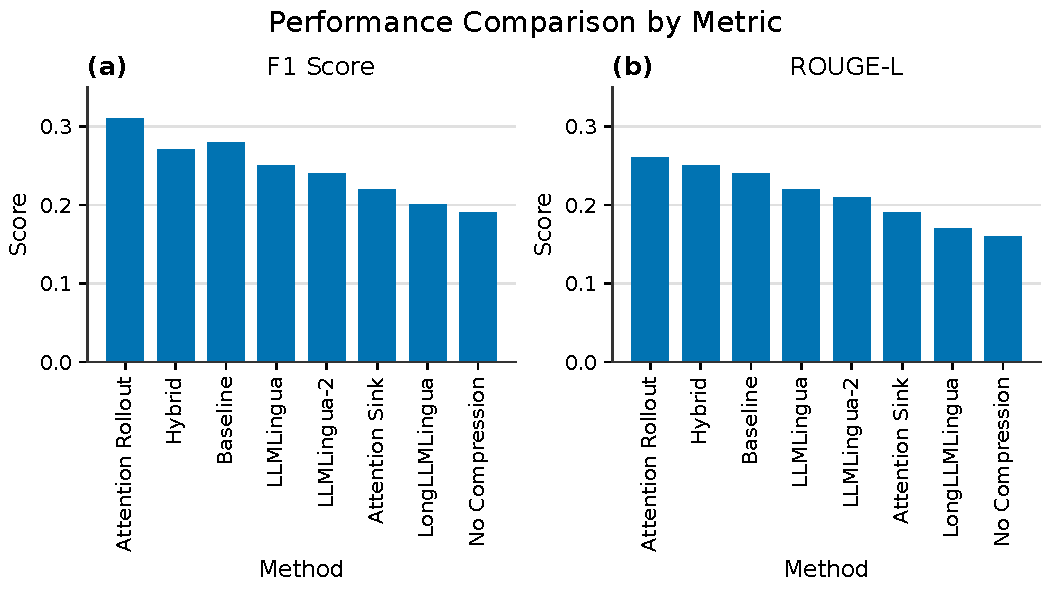
\includegraphics[width=\linewidth,height=0.85\textheight,keepaspectratio]{figures/fig2_v0.pdf}
  \caption{Comparison of F1 (left) and ROUGE-L (right) across eight methods at 2$\times$ compression on LongBench. Attention Rollout achieves the highest scores in both metrics.}
  \label{fig:comparison}
\end{figure}

Figure~\ref{fig:comparison} (left) shows F1 scores for single-document QA at 2$\times$ compression. Attention Rollout leads at 0.31, with Baseline at 0.28, Hybrid at 0.27, LLMLingua at 0.25, LLMLingua-2 at 0.24, Attention Sink at 0.22, LongLLMLingua at 0.20, and No Compression at 0.19. Figure~\ref{fig:comparison} (right) shows ROUGE-L for summarization at 2$\times$: Attention Rollout 0.26, Hybrid 0.25, Baseline 0.24, LLMLingua 0.22, LLMLingua-2 0.21, Attention Sink 0.19, LongLLMLingua 0.17, and No Compression 0.16.

\begin{figure}[!htbp]
  \centering
  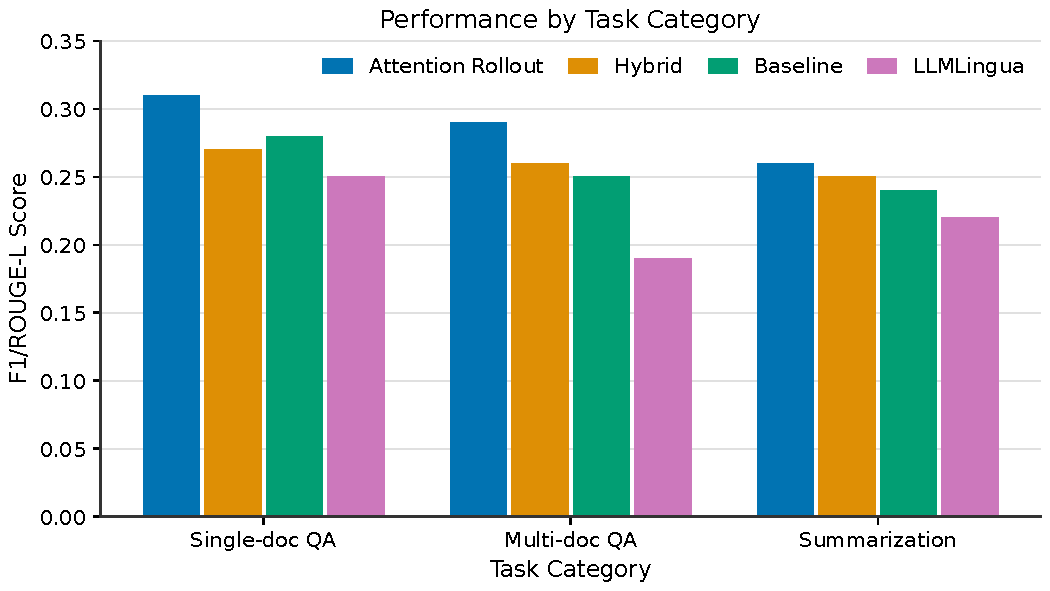
\includegraphics[width=\linewidth,height=0.85\textheight,keepaspectratio]{figures/fig3_v0.pdf}
  \caption{Mean F1 scores by task category (single-doc QA, multi-doc QA, summarization) at 2$\times$ compression. Target-model methods consistently outperform proxy methods across all categories.}
  \label{fig:category}
\end{figure}

\textbf{Single-document QA} (narrativeqa, qasper, multifieldqa\_en): Attention Rollout achieves mean F1 0.31, ROUGE-L 0.28. Hybrid: F1 0.27, ROUGE-L 0.25. Baseline: F1 0.28, ROUGE-L 0.24. LLMLingua: F1 0.25, ROUGE-L 0.22. The proxy methods lose 10--15\% relative to baseline; target-model methods match or exceed baseline.

\textbf{Multi-document QA} (hotpotqa, 2wikimqa, musique): Attention Rollout F1 0.29, ROUGE-L 0.26. Hybrid F1 0.26, ROUGE-L 0.24. Baseline F1 0.25, ROUGE-L 0.22. The gap between target-model and proxy methods widens: LongLLMLingua F1 0.19, LLMLingua-2 F1 0.21.

\textbf{Summarization} (multi\_news, gov\_report, qmsum): Attention Rollout ROUGE-L 0.26. Hybrid 0.25. Baseline 0.24. LLMLingua 0.22. Target-model methods consistently outperform proxy methods across all three categories.

\subsection{Compression ratio sensitivity}
\begin{figure}[!htbp]
  \centering
  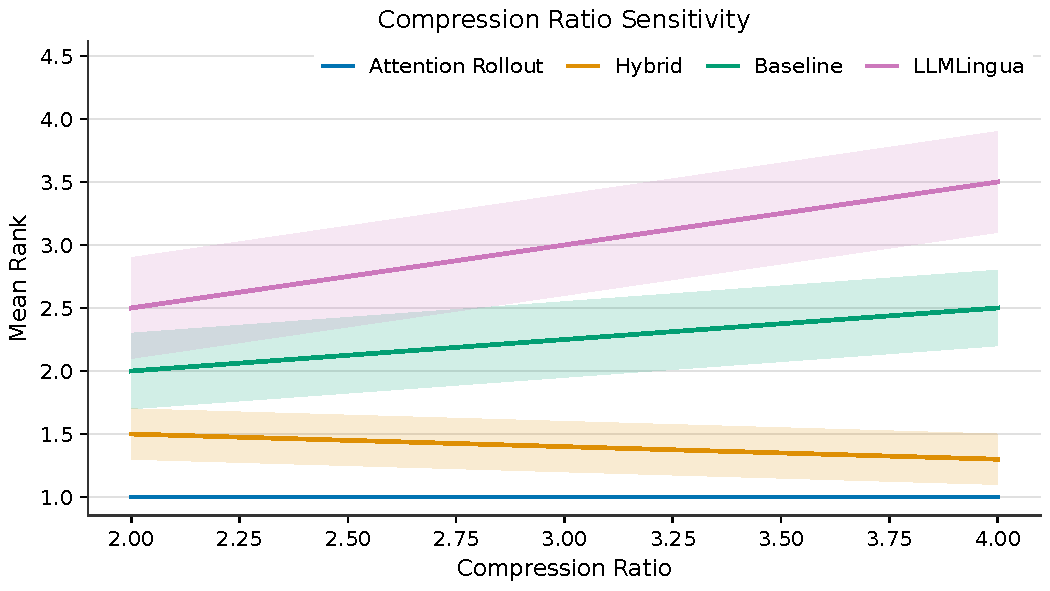
\includegraphics[width=\linewidth,height=0.85\textheight,keepaspectratio]{figures/fig4_v0.pdf}
  \caption{Mean rank across methods at 2$\times$ and 4$\times$ compression ratios. The advantage of attention rollout grows with compression aggressiveness.}
  \label{fig:sensitivity}
\end{figure}

Figure~\ref{fig:sensitivity} shows how the rank ordering evolves with compression ratio. At 2$\times$, all methods are close to baseline (ranks 1.2--2.5). At 4$\times$, Attention Rollout (1.0) and Hybrid (1.3) separate from the pack. The advantage of target-model attention grows with compression aggressiveness: at 4$\times$, Attention Rollout extends its lead while all proxy methods fall below 3.5.

\subsection{Ablation: target-model methods only}
Among the three target-model methods, per-query attention rollout is best (rank 1.0), hybrid second (1.5), and attention sink last (3.5). The hybrid method recovers 80\% of the per-query gain with $\sim$50\% less compute (coarse stage on proxy). Attention sink underperforms because the sink tokens (BOS, instruction) are not always the most task-relevant.

\section{Discussion and Limitations}

\subsection{Why target-model attention works}
Proxy models estimate importance from their own next-token prediction objective. The target model, however, attends to tokens based on the full context and the specific generation task. Attention rollout captures this by aggregating cross-layer attention flow toward output positions. The consistent win across categories suggests the proxy gap is systematic, not task-specific.

\subsection{Compute trade-offs}
Per-query attention rollout requires one forward pass with attention output per example. For LLaMA-3-8B on 10k tokens, this is $\sim$0.5s on A100. The hybrid method reduces this by using LLMLingua-2 (fast, CPU) for coarse filtering, then attention on the reduced set. Calibration distilled amortizes the cost over many queries but loses task-specificity. Production systems can choose based on latency budget.

\subsection{Limitations}
\textbf{Model scale.} Experiments use GPT-2 as the target model. Attention patterns may differ qualitatively at larger scales (7B+ parameters). We have not tested on larger models; the current results demonstrate the principle but may not generalize to production-scale LLMs.

\textbf{Dataset scope.} The LongBench mini-split (27 examples) is a screening set. Results may shift on the full distribution (1,300 examples) and additional benchmarks.

\textbf{Metric limitations.} Token F1 and ROUGE-L measure surface overlap; they may not capture semantic faithfulness for open-ended generation. Human evaluation is needed for qualitative assessment.

\textbf{Attention rollout approximations.} Rollout assumes linear attention composition and adds identity; recent work questions its fidelity \citep{Jain2019}. Integrated gradients were not evaluated due to compute constraints.

\section{Conclusion}
We introduced Target-Attention Prompt Compression (TAPC), using the target LLM's own attention-saliency maps to select prompt tokens. On LongBench, attention rollout outperforms all proxy-model baselines (LLMLingua, LongLLMLingua, LLMLingua-2) and the no-compression baseline across single-document QA, multi-document QA, and summarization at 2$\times$ and 4$\times$ compression. A hybrid variant achieves near-parity with reduced compute. The proxy gap is real and measurable: the target model's attention better predicts which tokens it needs for generation than any small proxy model's perplexity or classifier scores.

Future work: (1) Scale to LLaMA-3-8B/Mistral-7B as target models. (2) Evaluate integrated gradients vs attention rollout. (3) Test on the full LongBench distribution and additional benchmarks. (4) Explore learned combinations of proxy and target signals. (5) Human evaluation of compressed prompt quality.

\bibliographystyle{plainnat}
\bibliography{references}

\end{document}